\documentclass{article}
\usepackage[utf8]{inputenc}
\usepackage{csquotes}
\usepackage[british]{babel}
\usepackage{graphicx}
\usepackage{caption}
\usepackage{subcaption}
\usepackage[style=numeric, sorting=none, defernumbers=true]{biblatex}
\usepackage{hyperref}
\hypersetup{
    colorlinks=false
}

\addbibresource{references.bib}

\graphicspath{{./images/}}

\title{Asynchronous Multiplayer In Video Games}
\author{Hayley Davies - 1902055}
\date{27th March 2022}

\begin{document}

\maketitle

\section{Abstract}
[QUICKLY SUMMARISE THE OVERALL PAPER AND WHAT IS CONCLUDED]

\section{Introduction}
This paper serves to provide information regrding how a game's players can network asynchronously and how that can be used to create unique gameplay elements which entice the player.

For the paper, a game called \emph{War and Legacy} has been developed to demonstrate how asynchronous gameplay in video games can be utilised. This game works similar to Reigns\cite{reigns2016} in its card based, choose your own adventure style gameplay, where a player rules a kingdom a must try to not be overthrown by various hazards within the game. These hazards are Population, Military Strength and Financial Stability of the kingdom.

\section{Research}
Asynchronous multiplayer is defined by Ian Bogost\cite{bogost2004} with four primary principles.
\begin{enumerate}
    \item \emph{Asynchronous play supports multiple players playing in sequence, not in tandem}
    \item \emph{Asynchronous play requires some kind of persistent state which all players affect, and which in turn affects all players}
    \item \emph{Breaks between players are the organizing principle of asynchronous play}
    \item \emph{Asynchronous play need not be the defining characteristic of a game}
\end{enumerate}

Bogost goes on to list a multitude of both physical and digital games which have a asynchronous multiplayer element to them, many of which, such as Diplomacy\cite{diplomacy1959}, can also be played synchronously, or live, amongst its players.

There are various types of networked architecture within computer science, however, the main two are peer-to-peer networks and client-server networks.
\begin{figure}[!h]
    \centering
    \begin{subfigure}[b]{5cm}
        \centering
        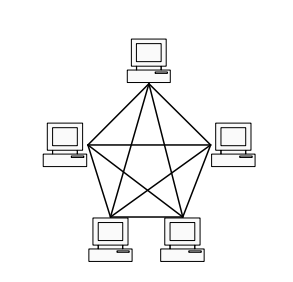
\includegraphics[width=5cm]{peer-to-peer.png}
        \caption{Peer-to-Peer}
    \end{subfigure}
    \begin{subfigure}[b]{5cm}
        \centering
        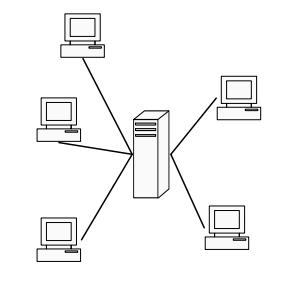
\includegraphics[width=5cm]{client-server.png}
        \caption{Client-Server}
    \end{subfigure}
    \caption{Chia-chun Hsu 2003. Topology for Multiplayer Online Game system. [digital]}
\end{figure}

Peer-to-peer is defined by Schollmeier\cite{schollmeier2001} as a network where "the participants share a part of their own hardware resources [which are] necessary to provide the service and content ... without passing [through] intermediary entities." The popular torrent protocol is based on this principle.

Peer-to-peer is then further split into two classifications by Schollmeier; "Pure" and "Hybrid". Pure peer-to-peer is where "any single, arbitrary chosen [peer] can be removed from the network without [it] sufffering any loss of network service." Hybrid peer-to-peer is where "a central entity is necessary to provide parts of the offered network services."

Schollmeier defines Client-Server network as a server where the client and server are two distinct nodes where "a client only requests content" and "the server is the only ... provider of content."

Within a video games context, both peer-to-peer and client-server networks are utilised. Hsu compares both systems\cite{hsu2003} with six characteristics; Scalability, Delay, Robustness, Consistency, Cheat-proof and Easy to charge. They conclude that peer-to-peer is good for Robustness, Scalability and Delay, but poor for Consistency, Cheat-proof and Easy to charge, whereas, Client-Server is the opposite, being poor for Robustness, Scalability and Delay, but good for Consistency, Cheat-proof and Easy to charge.

[ADD MORE RESEARCH ABOUT NETWORKING SOLUTIONS]

\section{System}
For War and Legacy the gameplay revolves around asynchronous interaction between players. This is difficult to achieve in a peer-to-peer networked system as players within War and Legacy never directly at the same time. As such, for this type of project, a client-server network solution works better as you can ensure consistency between players.

[TALK MORE ABOUT THE SYSTEM I PLAN ON USING WITH WAR AND LEGACY]

\section{Conclusion}
[CONCLUDE SOMETHING]

\defbibfilter{papers}{
    type=inproceedings or
    type=article or
    type=book
}

\printbibliography[filter=papers]
\printbibliography[type=software, title={Games}]

\listoffigures

\end{document}